%%%%%%%%%%%%%%%%%%%%%%%%%%%%%%%%%%%%%%%%%%%%%%%%%%%%%%%%%%
%%
%% MARK: Title
%%
%%%%%%%%%%%%%%%%%%%%%%%%%%%%%%%%%%%%%%%%%%%%%%%%%%%%%%%%%%

\chapter*{\S B9. On Riemannian Metric in Diffeology}
\setcounter{footnote}{0}

\begin{abstract}
  In this note,
  we attempt to establish the formal framework of Riemannian diffeology.
  This involves providing a definition of a Riemannian metric that coincides with the standard definition on manifolds.
  It is easy to define a symmetric,
  covariant positive 2-tensor;
  the tricky part is deciding what we mean by positive definite.
\end{abstract}

In what follows,
I have chosen to adopt a point-wise approach to defining a Riemannian metric on diffeological spaces.

%%%%%%%%%%%%%%%%%%%%%%%%%%%%%%%%%%%%%%%%%%%%%%%%%%%%%%%%%%
%%
%% MARK: Pointed or pointwise diffeology
%%
%%%%%%%%%%%%%%%%%%%%%%%%%%%%%%%%%%%%%%%%%%%%%%%%%%%%%%%%%%
\section{Pointed or pointwise diffeology}

The notion of pointed or pointwise diffeology has been used in a few places already:
for the dimension in diffeology \cite[\textsection\,2.19/20]{PIZ13},
and for the construction of differential $p$-form bundles and $p$-vector bundles (op.\,cit. \textsection\,6.45).
We can detach the definition of pointwise diffeological objects from an ambient diffeology,
and make it depend solely on a pointed diffeology.
First,
let us recall:

\begin{Article}{Pointed parametrization.}{}
  A \emph{pointed parametrization} in a set $X$ at a point $x$ is any parametrization $P :U \to X$ such that:
  $0 \in U$ and $P(0)=x$.
  We denote by $\Params_x(X)$ the set of all parametrizations pointed at $x$.
\end{Article}

\begin{Article}{Pointed diffeology.}{}
  Let $X$ be a set and $x \in X$.
  We call a \emph{pointed diffeology} at $x$ any set $\cD_x \subset \Params_x(X)$ that satisfies the two axioms:
  
  \begin{enumerate}
    \item The constant parametrization $0 \mapsto x$ belongs to $\cD_x$.
    \item For all parametrization $P : U \to X$ belonging to $\cD_x$ and for all smooth parametrization $F : V \to U$,
    pointed at $0$,
    $P \circ F$ belongs to $\cD_x$.
  \end{enumerate}
\end{Article}

Note that a pointed diffeology at $x$ is always the germ at the point $x$ of the diffeology it generates (op.\,cit. \textsection\,1.6).
And,
for any diffeology $\cD$,
the subset $\cD_x \subset \cD$ of plots pointed at $x$ is a pointed diffeology.

\begin{Article}{Pointed path.}{}
  A pointed path at $x \in X$ is a pointed smooth parametrization at $x$,
  defined on $\RR$ or some interval $]a,b[$.
\end{Article}

\begin{Article}{Pointed $p$-form.}{}
  \emph{A pointed $p$-form} at $x$ is a map $\alpha_x$ that associates to every pointed plot $P$ at $x$ a linear $p$-form $\alpha_x(P) \in \Lambda^p(\RR^n)$ at $0 \in \Domain(P) \subset \RR^n$,
  such that $\alpha_x(P \circ F) = F^*(\alpha_x(P))_0$,
  that is:
  \begin{align*}
    \alpha_x(P \circ F)(v_1,\ldots,v_p) & = \alpha_x(P)(M v_1,\ldots,M v_p),\\
    & \text{with} \ M = \Der(F)(0),
  \end{align*}
  for all smooth parametrization $F$ in $\Domain(P)$ pointed at $0$.
  We shall denote the space of pointed $p$-forms at $x$ by ${\blambda}^p_x(X)$.
  
  \Note The value at $x$ of a (global) $p$-form is a pointed $p$-form,
  but not every pointed $p$-form is the value of a (global) $p$-form.
  
  We have denoted by $\Lambda_x^p(X)$ the space of values of $p$-forms at $x$ (op.\,cit. \textsection\,6.45).
  According to our notations:
  $
    \Lambda_x^p(X) \subset \lambda_x^p(X).
    $
\end{Article}

%%%%%%%%%%%%%%%%%%%%%%%%%%%%%%%%%%%%%%%%%%%%%%%%%%%%%%%%%%
%%
%% MARK: Smooth covariant tensor
%%
%%%%%%%%%%%%%%%%%%%%%%%%%%%%%%%%%%%%%%%%%%%%%%%%%%%%%%%%%%
\section{Smooth covariant tensor}

We recall (op.\,cit. \textsection\,6.20 Note, 6.21) that a \emph{smooth covariant tensor} on a diffeological space is a map $\epsilon$ that associates to every plot $P$ in $X$ a smooth covariant tensor $\epsilon(P)$ on $U = \Domain(P)$,
such that
$$
  \epsilon(P \circ F) = F^*(\epsilon(P))
  $$
for all smooth parametrization $F : V \to U$.
The tensor $\epsilon$ is symmetric if $\epsilon(P)$ is symmetric for all $P$.
In what follows we deal with symmetric $2$-tensors and we denote their space by
$$
  \Sigma^2(X),
  $$
and the space of symmetric $2$-tensors on a Euclidean subset $U$ by $\Sigma^2(U)$ with the identification $\epsilon \sim \epsilon(\Id_U)$.

Regarding notation: if $\epsilon$ is a smooth covariant $k$-tensor on a domain $U \subset \RR^n$,
we denote by $\epsilon_r(v_1,\ldots,v_k)$ the evaluation of $\epsilon$ at the point $r \in U$,
applied to the $k$-tuple of vectors $v_1,\ldots,v_k \in \RR^n$.
For $n=1$,
a vector is just a number and $1$ is the canonical basis vector.

%%%%%%%%%%%%%%%%%%%%%%%%%%%%%%%%%%%%%%%%%%%%%%%%%%%%%%%%%%
%%
%% MARK: Riemannian metric on a diffeological space
%%
%%%%%%%%%%%%%%%%%%%%%%%%%%%%%%%%%%%%%%%%%%%%%%%%%%%%%%%%%%
\section{Riemannian metric on a diffeological space}

\begin{Article}{Riemannian metric.}{}
  We shall define,
  for now,
  a Riemannian metric on a diffeological space $X$ as a covariant $2$-tensor that satisfies the following conditions:
  
  \begin{itemize}
    \item (Symmetric) The tensor $g$ is symmetric:
    $$
      g \in \Sigma^2(X).
      $$
    %
    \item (Positive) For all paths $\gamma \in \Paths(X)$,
    $g(\gamma) \geq 0$,
    that is
    $$
      g(\gamma)_t(1)(1) \geq 0 \quad \text{for all $t\in \RR$}.
      $$
    Actually we can restrict to paths defined on $\RR$ or on intervals $]a,b[$;
    in that case $g(\gamma)_t(1)(1) \geq 0$ for all $t \in \Domain(\gamma)$ obviously.
    %
    \item (Definite) The tensor $g$ is positive definite:
    $$
      g(\gamma)_t(1)(1) = 0 \quad \text{if and only if} \quad \forall \alpha \in \DForms^1(X), \ \alpha(\gamma)_t(1) = 0.
      $$
  \end{itemize}
\end{Article}

The last condition can be weakened by considering pointed differential forms,
as defined above.
Considering the space $\lambda^k_x(X)$ of pointed $k$-forms at $x$,
the positivity condition becomes:

\begin{itemize}
  \item {\it {\upshape(Definite')} The tensor $g$ is positive definite if for every point $x \in X$,
  for every path $\gamma$ pointed at $x$:
  $$
    g(\gamma)_0(1)(1) = 0 \quad \text{if and only if} \quad \forall \alpha_x \in \lambda_x^1(X), \ \alpha_x(\gamma)_0(1) = 0.
    $$
  }
\end{itemize}

It is not clear which definition is best,
for many examples built with manifolds and spaces of smooth maps they coincide.
But they may differ in general and, depending on the problem, one must choose one or the other.

\begin{Article}{Length and energy of a path.}{}
  Let $g$ be a Riemannian metric on a diffeological space $X$.
  For any path $\gamma$ in $X$,
  we define its \emph{length} and its \emph{energy} by:
  $$
    \Length(\gamma) = \int_0^1 \sqrt{g(\gamma)_t(1)(1)} \,\dt,
    \quad \text{and} \quad
    E(\gamma) = {1\over 2} \int_0^1 g(\gamma)_t(1)(1) \,\dt.
    $$
\end{Article}

%%%%%%%%%%%%%%%%%%%%%%%%%%%%%%%%%%%%%%%%%%%%%%%%%%%%%%%%%%
%%
%% MARK: How does this fit?
%%
%%%%%%%%%%%%%%%%%%%%%%%%%%%%%%%%%%%%%%%%%%%%%%%%%%%%%%%%%%
\section{How does this fit?}

\begin{Article}{Exercise 1.}{}
  For $x \in X$ we say that a path $\gamma$ is centered at $x$ if $\gamma(0) = x$.
  Let $g$ be a symmetric $2$-tensor on $X$.
  Show that:
  
  \begin{itemize}
    \item $g$ is positive if for all $x \in X$,
    for all paths $\gamma$ centered at $x$,
    $g(\gamma)_0(1)(1) \geq 0$.
    
    \item $g$ is definite if for all $x \in X$,
    for all paths $\gamma$ centered at $x$,
    $g(\gamma)_0(1)(1) = 0$ implies that for all $1$-forms $\alpha$ on $X$,
    pointed or not,
    $\alpha(\gamma)_0(1) = 0$.
  \end{itemize}
\end{Article}

\begin{proof}
  It is part of the definition that if $g(\gamma)_t(1)(1) \geq 0$ for all paths $\gamma$ in $X$ and all $t \in \Domain(\gamma)$,
  then,
  for all $x \in X$,
  for all paths $\gamma$ centered at $x$,
  $g(\gamma)_0(1)(1) \geq 0$.
  Conversely,
  assume that for all $x \in X$,
  for all paths $\gamma$ centered at $x$,
  $g(\gamma)_0(1)(1) \geq 0$.
  Let $\gamma'$ be a path in $X$ and $t \in \Domain(\gamma')$,
  and let $x = \gamma'(t)$.
  Let $\Trsl_{t}(t') = t' + t$ be the translation by $t$ in $\RR$ and set $\gamma = \gamma' \circ \Trsl_{t}$.
  Then,
  \begin{align*}
    g(\gamma)_0(1)(1) & = g(\gamma' \circ \Trsl_{t})_0(1)(1) \\
    & = \Trsl_{t}^*(g(\gamma'))_0(1)(1) \\
    & = g(\gamma')_t(1)(1) \qquad \text{because $\Der(T_t)_0(1) = 1$.}
  \end{align*}
  Thus,
  for all $t \in \Domain(\gamma')$,
  $g(\gamma')_t(1)(1) \geq 0$.
  
  The same use of translation by $t$ proves the second proposition.
\end{proof}

\begin{Article}{Exercise 2.}{}
  Show that when $X = M$ is a manifold,
  this definition coincides with the standard definition.
  We choose the definition of positive definite metric with pointed forms.
  Explain why on a manifold the two conditions coincide.
\end{Article}

\begin{proof}
  Let $\cA$ be an atlas of $M$ and let $\dim(M) = n$.
  By definition,
  for every chart $F \in \cA$,
  %%###########
  \begin{figure}[tb]
    \centerline{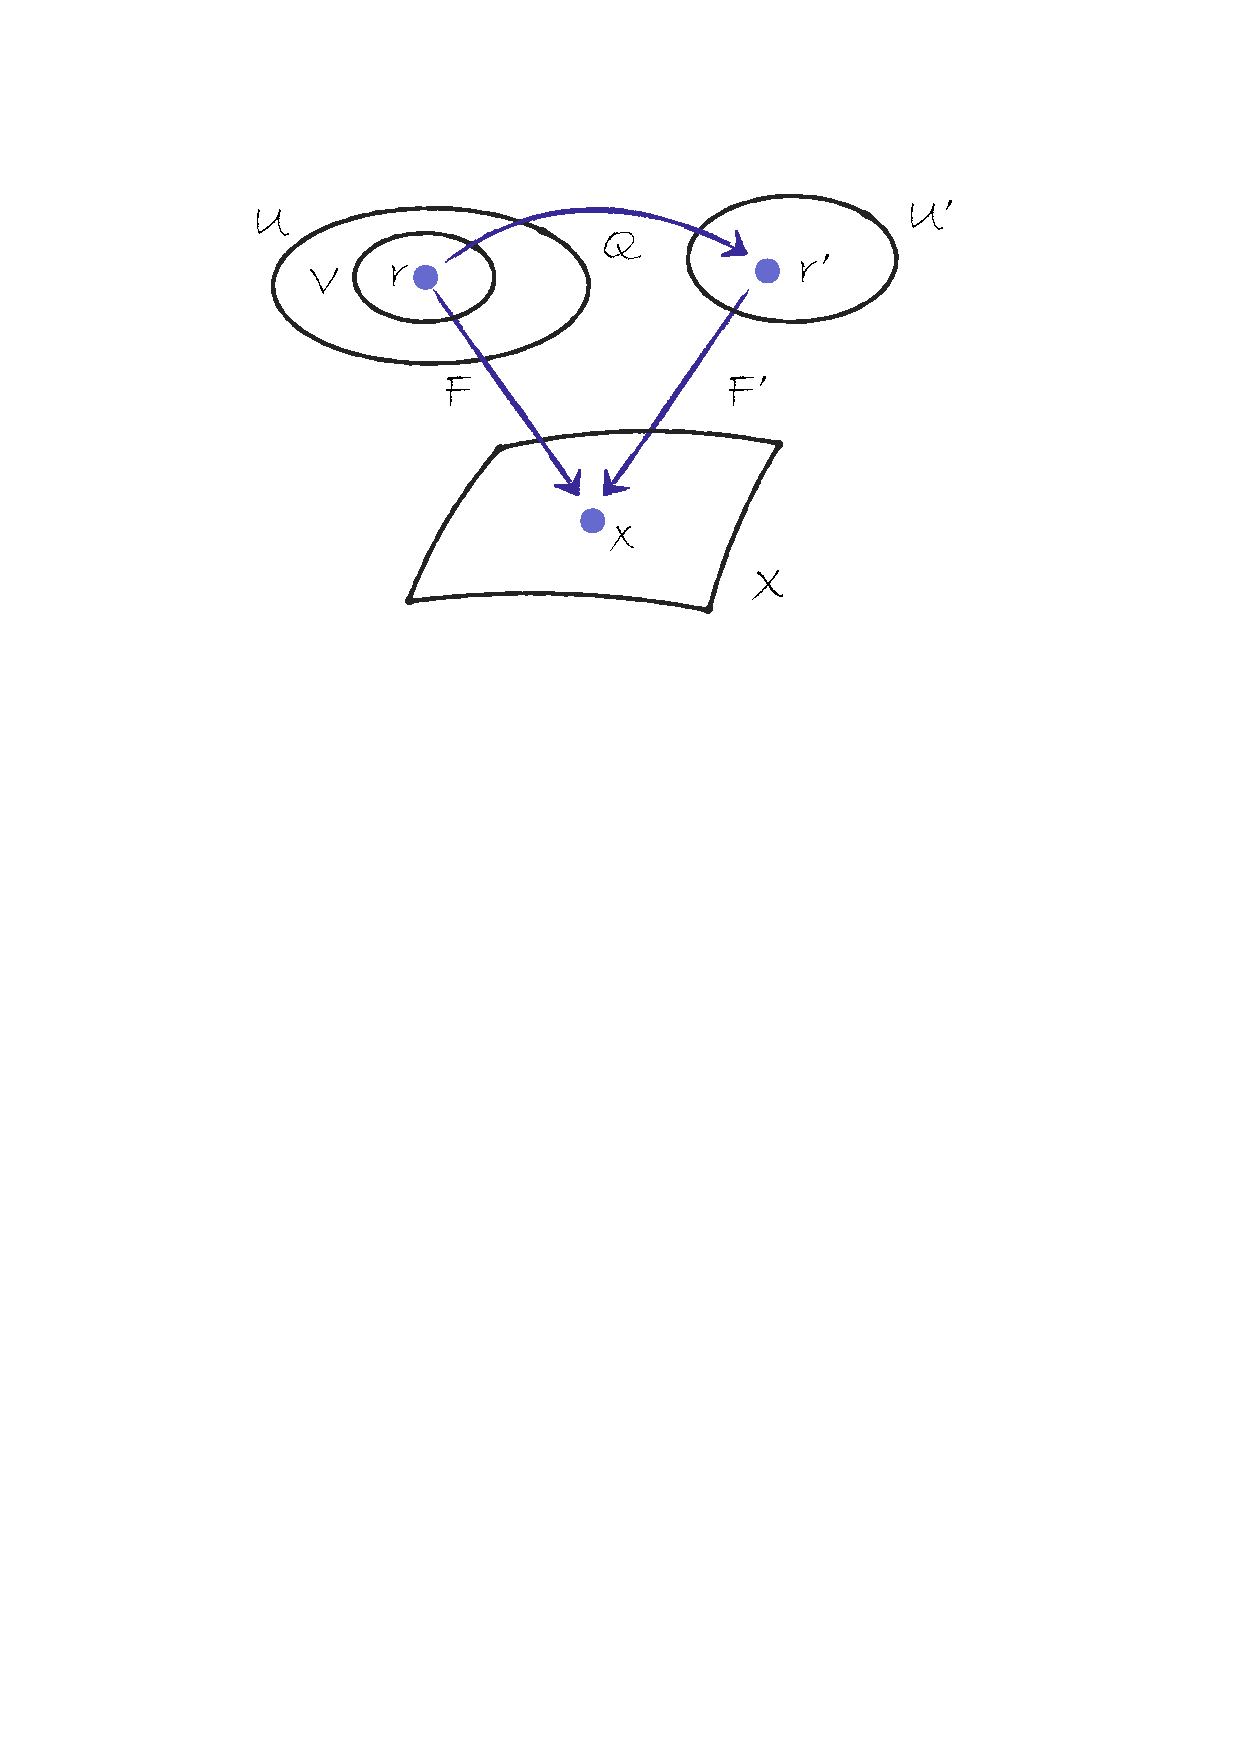
\includegraphics[width=.5\textwidth]{Figures/fig-transition-function.pdf}}
    \vspace{-.5ex}
    \caption{The transition function.}
    \label{fig-transition-function}
  \end{figure}
  %%###########
  $g(F)$ is a symmetric $2$-tensor on $\Domain(F)$,
  since a chart is a particular plot.
  Let $x \in M$ and two charts $F,F' \in \cA$ such that $F(r) =F'(r')=x$.
  Since $\cA$ is a generating family,
  there exists an open neighborhood $V \subset \Domain(F)$ of $r$ and a plot $Q :V \to\Domain(F')$ such that $F' \circ Q = F \restriction V$,
  $Q(r) = r'$,
  and we can choose $V$ such that $Q(V) \subset \Domain(F')$.
  Thus,
  $g(F \restriction V) = g(F \circ Q) = Q^*(g(F'))$,
  but $Q = F'^{-1} \circ F \restriction V$ is the transition diffeomorphism,
  hence:
  $g(F) = (F'^{-1} \circ F)^*(g(F'))$, which is the definition of a $2$-tensor on a manifold.
  
  Now,
  let $F$ be a chart of $M$.
  As we said, $g(F)$ is a symmetric $2$-tensor on $\Domain(F)\subset \RR^n$.
  Let $g(F)_r$ be its value at $r$,
  and $x = F(r)$.
  Let $v \in \RR^n$ and $\gamma_v : t \mapsto r + tv$,
  $\gamma_v$ is a smooth path in $\Domain(F)$,
  defined on some interval in $\RR$ and centered at $r$.
  Let $\gamma^v = F \circ \gamma_v$,
  then $\gamma^v(0) = F(r)= x$.
  Then:
  \begin{align*}
    g(\gamma^v)_0(1)(1) & = g(F \circ \gamma_v)_0(1)(1) \\
    & = \gamma_v^*(g(F))_0(1)(1) \\
    & = g(F)_{\gamma_v(0)}(\dot\gamma_v(0),\dot\gamma_v(0)), \quad \text{with } \dot\gamma_v(t) = {d\gamma_v(t) \over dt}\\
    & = g(F)_r(v,v)
  \end{align*}
  Since $g(\gamma)_0(1)(1) \geq 0$ for all $\gamma$,
  then,
  for $\gamma = \gamma^v$,
  $g(F)_r(v,v) \geq 0$ for all $r \in \Domain(F)$ and $v \in \RR^n$.
  Thus,
  $g(F)$ is a non-negative symmetric $2$-tensor.
  
  Now,
  let $F$ be a chart and let us check that $g(F)$ is positive definite.
  Let $r \in \Domain(F)$ and $v \in \RR^n$.
  Let $x = F(r)$.
  Assume that $g(F)_r(v,v) = 0$.
  Let $\gamma_v(t) = r + tv$ and $\gamma^v = F \circ \gamma_v$,
  then:
  \begin{align*}
    g(F)_r(v,v)  & = g(F)_{\gamma_v(0)}(\dot\gamma_v(0),\dot\gamma_v(0)) \\
    & = \gamma_v^*(g(F))_0(1)(1) \\
    & = g(F \circ \gamma_v)_0(1)(1) \\
    & =  g(\gamma^v)_0(1)(1)
  \end{align*}
  So,
  if $g(F)_r(v,v) = 0$ then $g(\gamma^v)_0(1)(1) = 0$,
  which implies,
  by hypothesis,
  that for every $1$-form $\alpha_x$ pointed at $x$,
  $\alpha_x(\gamma^v) = 0$.
  Consider now the coordinate $1$-forms $e_i^*: v \mapsto v^i$,
  for $v = \sum_i v^i e_i$,
  where $(e_i)_{i=1}^n$ is the canonical basis of $\RR^n$.
  Push the form $e_i^*$ onto $M$ by the chart $F$:
  %%###########
  \begin{figure}[b]
    \centerline{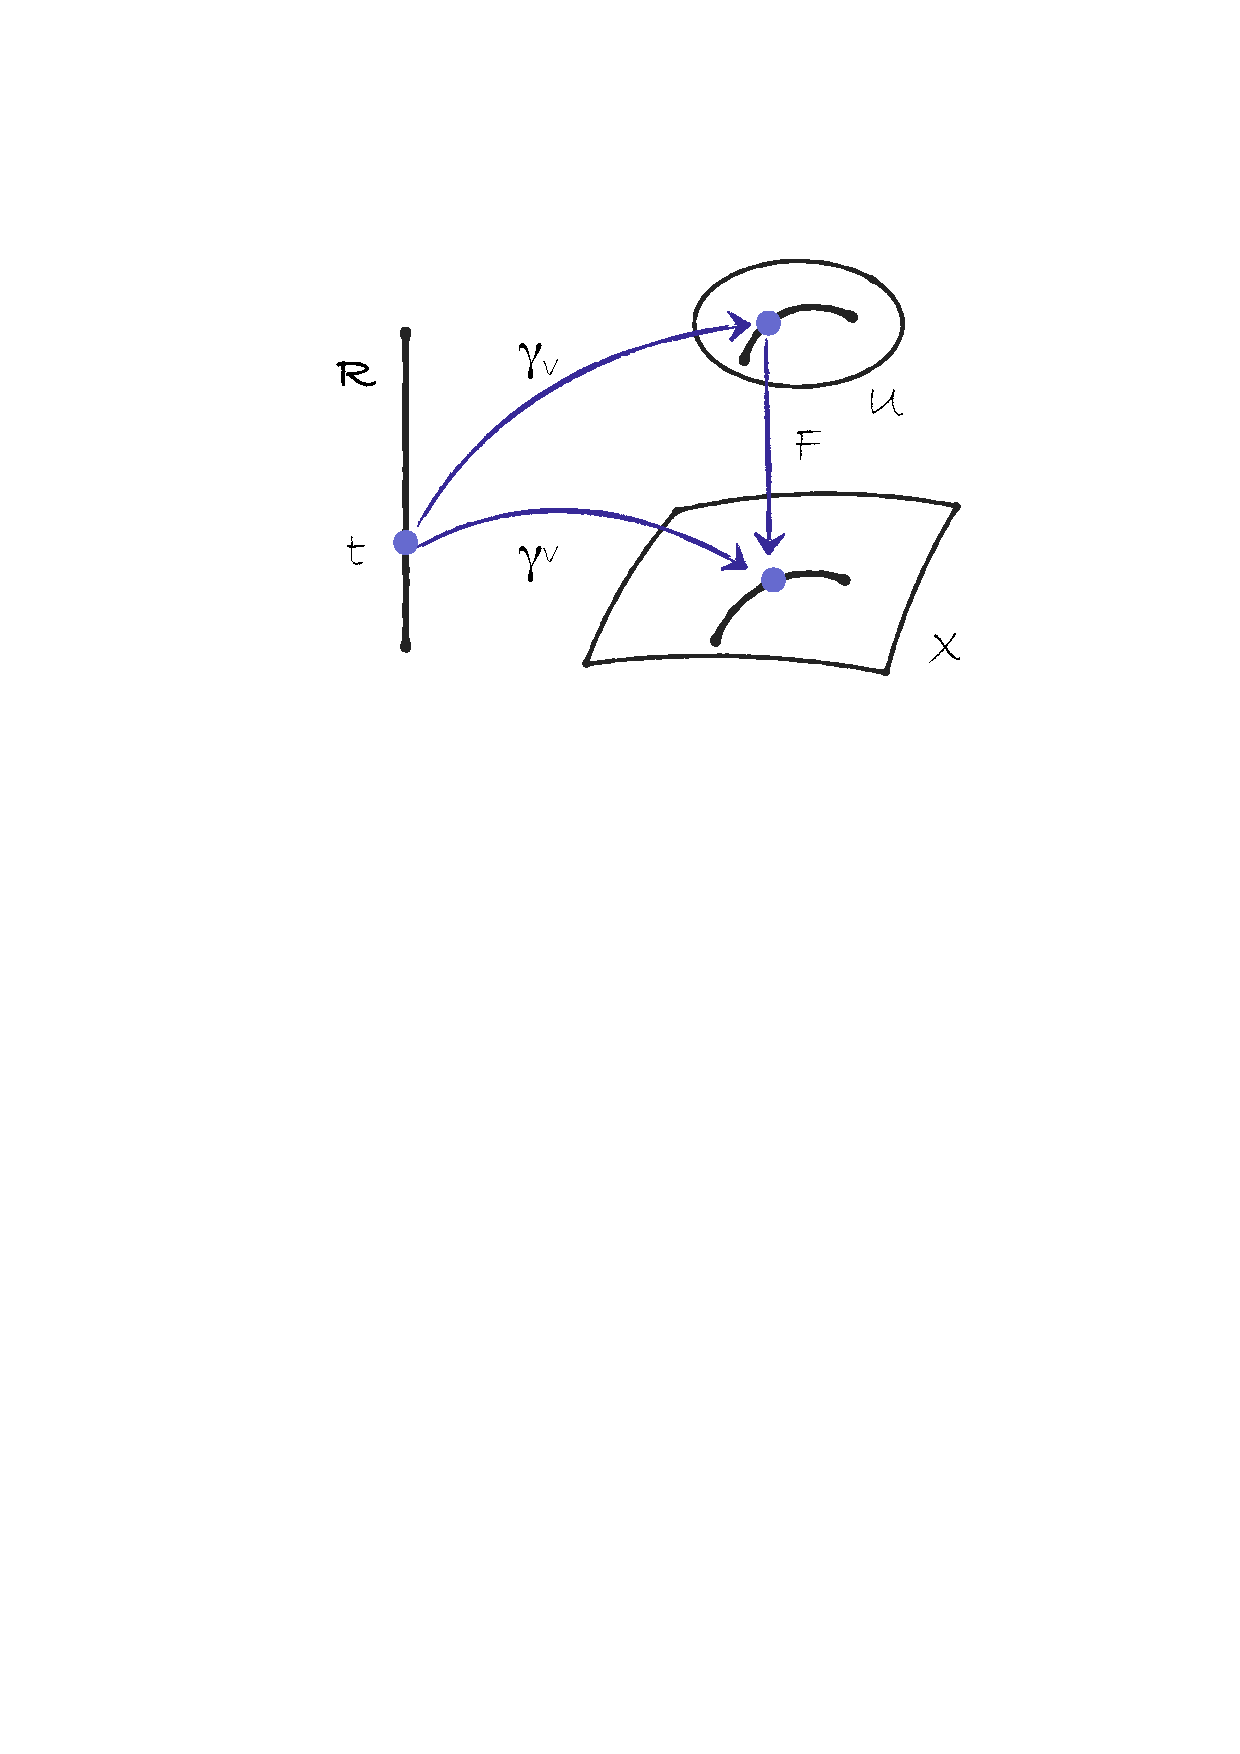
\includegraphics[width=.5\textwidth]{Figures/fig-path-manifold.pdf}}
    \vspace{-.5ex}
    \caption{A path in a chart.}
    \label{fig-path-manifold}
  \end{figure}
  %%###########
  Define $\epsilon_i^x$ as follows:
  for every plot $P : U \to X$ pointed at $x$,
  there exists a smooth parametrization $Q$ pointed at $r$,
  with $F(r)= x$,
  defined on a neighborhood $V$ of $0 \in U$ such that $P \restriction V = F \circ Q$.
  Then,
  let $\epsilon_i^x(P) = Q^*(e_i^*)$;
  this is a $1$-form centered at $x$.
  Indeed,
  for $P' = P \circ F$,
  $Q' = Q \circ F$ and $\epsilon_i^x(P \circ F) = (Q \circ F)^*(e_i^*) = F^*(Q^*(e_i^*)) = F^*(\epsilon_i^x(P))$.
  Now,
  since $g$ is assumed to be positive definite:
  $\epsilon_i^x(\gamma^v) = 0$,
  but $\gamma^v = F \circ \gamma_v$,
  thus $\epsilon_i^x(\gamma^v) = \gamma_v^*(e_i^*) = (e_i^*)_r(\dot\gamma_v(0)) = e_i^*(v) = v^i$.
  Hence,
  for all $i$,
  $v^i = 0$ and then $v = 0$.
  The $2$-tensor $g(F)$ defined on $\Domain(F)$ is a positive definite metric.
\end{proof}

\begin{Article}{Exercise 3.}{}
  For two vectors $v,v' \in \RR^3$,
  denote by $\langle v, v' \rangle$ their ordinary scalar product.
  Let $\gamma \in \Paths(\RR^3)$,
  and call a \emph{variation} of $\gamma$ a path $t \mapsto (x_t,v_t)$ such that $x_t = \gamma(t)$ and $v_t \in \RR^3$.
  For two variations $\nu = [t \mapsto (x_t,v_t)]$ and $\nu' = [t \mapsto (x_t,v'_t)]$ of $\gamma$,
  define the product
  $$
    \langle \nu,\nu' \rangle = \int_0^1 \langle v_t,v'_t\rangle \, \dt.
    $$
  
  \Question{\bf Q1.} Consider this product as defining a formal Riemannian metric on $\Paths(\RR^3)$.
  
  \Question{\bf Q2.} Compute explicitly the energy of a path $[s \mapsto \gamma_s]$ in $\Paths(\RR^3)$.
\end{Article}

\begin{proof}
  Let $P: U \to \Paths(\RR^3)$ be an $n$-plot.
  Define $g(P)$ as a $2$-tensor on $U$ by:
  for all $r \in U$ and $v,v' \in \RR^n$,
  $$
    g(P)_r(v,v') = \int_0^1 \left\langle {\partial \gamma_r(t) \over \partial r}(v), {\partial \gamma_r(t) \over \partial r}(v') \right\rangle \ \dt.
    $$
  Let us prove that $g$ is a Riemannian metric on $\Paths(\RR^3)$.
  Consider $g(P \circ F)$,
  with $F$ a smooth parametrization in $U$.
  Write $F :s \mapsto r$,
  $P : r \mapsto \gamma$ and then $P \circ F : s \mapsto \gamma$.
  We have:
  \begin{align*}
    g(P \circ F)_s(w,w') &  = \int_0^1 \left\langle {\partial \gamma(t) \over \partial s}(w), {\partial \gamma(t) \over \partial s}(w') \right\rangle \ \dt \\
    & = \int_0^1 \left\langle {\partial \gamma(t) \over \partial r}{\partial r \over \partial s}(w), {\partial \gamma(t) \over \partial r}{\partial r \over \partial s}(w')  \right\rangle \ \dt \\
  \end{align*}
  We recall that for a smooth parametrization $f : x \mapsto y$,
  where $x$ and $y$ are real variables,
  we use interchangeably the notations
  $$
    \Der(f) \quad \text{or} \quad \Der(x \mapsto y) \quad \text{or} \quad {\partial y \over \partial x}.
    $$
  Then for $g \circ f : x \mapsto y \mapsto z$,
  the chain rule gives:
  $$
    \Der(x \mapsto z) = \Der(x \mapsto y \mapsto z) = \Der(y \mapsto z) \circ \Der(x \mapsto x),
    $$
  or:
  $$
    {\partial z \over \partial x} = {\partial z \over \partial y} \circ  {\partial y \over \partial x}.
    $$
  Therefore,
  setting
  $$
    v = {\partial r \over \partial s}(w) \quad \text{and} \quad v' = {\partial r \over \partial s}(w'),
    $$
  we obtain:
  \begin{multline*}
    g(P \circ F)_s(w,w')   = \int_0^1 \left\langle {\partial \gamma(t) \over \partial r}{\partial r \over \partial s}(w), {\partial \gamma(t) \over \partial r}{\partial r \over \partial s}(w')  \right\rangle \dt \\
    = \int_0^1 \left\langle {\partial \gamma(t) \over \partial r}(v), {\partial \gamma(t) \over \partial r}(v') \right\rangle \dt \\
    = g(P)_{r = F(s)} \left({\partial F(s) \over \partial s}(w), {\partial F(s) \over \partial s}(w')\right)
    = F^*(g(P))_s(w,w').
  \end{multline*}
  Hence,
  $g$ is a covariant $2$-tensor on $\Paths(\RR^3)$.
  It is symmetric because the scalar product is symmetric.
  
  Now,
  let $s \mapsto \gamma_s$ be a path in $\Paths(\RR^3)$,
  \begin{equation*}
    g(s \mapsto \gamma_s)_s(1,1)   = \int_0^1 \left\langle {\partial \gamma_s(t) \over \partial s}, {\partial \gamma_s(t) \over \partial s} \right \rangle \ \dt
    = \int_0^1 \left\Vert{{\partial \gamma_s(t) \over \partial s}}\right\Vert^2 \ \dt.
  \end{equation*}
  Clearly $g(s \mapsto \gamma_s)_s(1,1)$ is positive.
  Now,
  $$
    g(s \mapsto \gamma_s)_s(1,1) = 0 \ \Rightarrow\ \left\Vert{{\partial \gamma_s(t) \over \partial s}}\right\Vert^2 = 0 \text{ for all } t.
    $$
  Hence,
  $$
    {\partial \gamma_s(t) \over \partial s} = 0 \ \Rightarrow\ \gamma_s = \gamma \text{ (constant in $s$)}.
    $$
  The path $s \mapsto \gamma_s$ is constant.
  Thus,
  for every $1$-form $\alpha$ on $\Paths(\RR^3)$,
  $\alpha(s \mapsto \gamma) = 0$,
  since differential forms vanish on constant plots (op.\,cit. Ex. 96).
  Therefore,
  the tensor $g$ defined on $\Paths(\RR^3)$ is positive and definite;
  it is a diffeological Riemannian metric according to the definition above.
  Hence,
  $$
    E(s \mapsto \gamma_s) = {1 \over 2} \int_0^1 \!\! \int_0^1 \left\Vert{{\partial \gamma_s(t) \over \partial s}}\right\Vert^2 \ \dt \,\ds
    $$
  is the energy of the path $s \mapsto \gamma_s$ in $\Paths(\RR^3)$.
\end{proof}
